
% Due Date: 7/14/14

\chapter{A Full-Scale Production Application: S3D}
\label{chapter:s3d}

Instead of evaluating Legion on many small benchmark
applications, we decided to evaluate Legion on a single 
full-scale production application. The reason for this
decision is two-fold.  First, evaluating Legion features
in isolation is difficult because many of them only make 
sense within the context of a Legion implementation. 
Testing our Legion implementation in an end-to-end fashion
at scale demonstrates that our design decisions lead
to an efficient implementation and that all components 
of Legion operate in concert to achieve high performance.

Our second reason for performing an end-to-end evaluation
of Legion at scale is that evaluating benchmarks at
smaller scales often fails to translate to high performance
for applications run over thousands of nodes
on real machines. At such scales, many features
of a system are tested and bottlenecks are discovered
that are not obvious at smaller scales. Due to this
phenomenon, we decided that a better evaluation of
the capability of Legion would be a comparison to 
an existing application written using current tools
that has been developed and optimized by experts.
By performing a comparison at full production
scale, we would truly test the advantages of the
Legion programming model.

For our comparison application we selected S3D 
\cite{S3D09}. S3D is a combustion simulation used
by researchers from the United States Department
of Energy to study the chemical and physical 
properties of fuel mixtures for internal combustion
engines. S3D simulates the turbulent processes 
involved in combustion by performing a direct
numerical simulation (DNS) of the Navier-Stokes
equations for fluid flow. The simulation for S3D
operates on regular Cartesian grid of points with
many values being stored on each point. The 
application iterates through time using a six 
stage, fourth order Runge-Kutta (RK) method. The 
RK method requires that the {\em right-hand side
function} (RHSF) be evaluated six times per
time step, requiring considerable computational
resources. There are many (often independent)
phases involved in computing the RHSF function
for all points, resulting in considerable task-
and data-level parallelism.

While the framework of S3D is general, S3D is
parametrized by the kind of {\em chemical 
mechanism} being simulated. A chemical mechanism
is constituted of a collection of species (molecules)
and reactions that govern the chemistry of the 
underlying simulation. For actual combustion, 
there are usually on the order of thousands of 
species and tens of thousands of reactions.
Performing a computational simulation of a
mechanism with perfect fidelity is computationally
intractable. Instead, {\em reduced} mechanisms
are developed that represent tractable approaches
to simulating combustion. Much of the original 
science done using S3D involved simulating the
{\tt H2} mechanism consisting of 9 chemical
species and 15 reactions. More recently S3D
is being used to simulate larger chemical 
mechanisms. Figure~\ref{fig:s3dmech} shows
details of the chemical mechanisms used for 
our experiments involving Legion. Each chemical
mechanism models a specific number of species
and reactions. In many cases, species with 
similar behavior are aliased resulting in a 
smaller number of {\em unique} species. In some
cases, certain groups of species need to appear
to be in a quasi-steady state, requiring a 
quasi-steady state approximation (QSSA). Additional
computation will be required for QSSA species.
Stiff species are those whose rates of change are
often volatile and are therefore subject to 
additional damping computations.

\begin{figure}
\centering
\begin{tabular}{c|ccccc}
Mechanism & Reactions & Species & Unique & QSSA & Stiff \\ \hline 
DME       &  175      &  39     &   30   &  9   &  22   \\ 
Heptane   &  283      &  68     &   52   &  16  &  27   \\ 
PRF       &  861      &  171    &   116  &  55  &  93   \\
\end{tabular}
\caption{Summary of Chemical Mechanisms Used in 
Legion S3D Experiments\label{fig:s3dmech}}
\end{figure}

S3D has been developed over the course of thirty
years by a number of scientists and engineers.
There are currently two primary versions of S3D.
The first version of S3D is the baseline version 
developed primarily by the scientists and is
used for active research. This version consists
of approximately 200K lines of Fortran code and
uses MPI \cite{MPI} for performing inter-node
communication when necessary. The choice of 
Fortran as the base language for S3D has allowed
scientists to take advantage of the many advances
made by Fortran compilers (developed by both
Cray and Intel) for generating both multi-threaded
and vectorized code. Many of the larger computational
loops are automatically partitioned across threads
and auto-vectorized leading to good performance
on homogeneous CPU-only clusters. While this version
of S3D was sufficient for performing science on
traditional clusters, it is challenging to scale
to modern machines and is currently unable to take
advantage of the heterogeneous processors (e.g. GPUs)
available on most modern supercomputers.

The second version of S3D developed more recently
combines MPI with OpenACC \cite{OpenACC} to target
modern heterogeneous supercomputers \cite{S3DACC12}.
This version of S3D was ported from the baseline
version by a team consisting of both scientists
as well as engineers from Cray and NVIDIA. By 
leveraging both CPUs and GPUs, this version of S3D
was made considerably faster than the baseline
version of S3D. Due to its higher performance
we chose this version of S3D to serve as our
baseline for performance comparisons with Legion.

In order to avoid porting all 200K lines of S3D 
into Legion, we decided instead to port the RHSF
function to Legion and leave the remaining 
start-up/tear-down code as well as the RK loop
in the original Fortran. The RHSF function represents
between 95-97\% of the execution for a time step
in S3D (depending on chemical mechanism and 
hardware), thereby representing the bulk of S3D's
computational workload. Ultimately we ported 
approximately 100K lines of Fortran into Legion
C++ code. By only porting a portion of S3D into
Legion, we also showcase Legion's ability to 
act as a library capable of inter-operating with
existing MPI code. By developing a path for
inter-operability we also demonstrate an 
evolutionary path for applications to be ported
into Legion that does not require all code to
be moved into Legion.

The rest of this chapter describes our implementation
of S3D in Legion. We begin by describing the 
machine-independent implementation of the S3D in
Legion based on logical regions and tasks in 
Section~\ref{sec:s3dimpl}. In this section we 
also describe how Legion is able to inter-operate
with MPI so only a portion of S3D is required to
be ported into Legion. We cover the details of 
how the Legion mapping interface allowed us to 
experiment with different mapping approaches in 
Section~\ref{sec:s3dmap}. Finally, we illustrate 
the performance benefits of Legion when compared to 
MPI and OpenACC in Section~\ref{sec:s3dperf}.

\section{S3D Implementation}
\label{sec:s3dimpl}
Our Legion implementation of the RHSF function in
S3D operates differently from a stand-alone Legion
application. Since most of the S3D code for starting
and analyzing an S3D run is in MPI-Fortran, we use
MPI to start-up a separate process on each 
node (in contrast to having GASNet start-up a process
on each node for the normal Legion initialization procedure).
Our Legion implementation of S3D is implemented as a 
library and we add a Fortran call into our library
that triggers the initialization of the necessary
data structures on each node. Consequently, Legion
is initialized within the same process as MPI. While
this is less than an ideal situation (we would have
preferred cooperating processes with isolation), 
alternative approaches are limited by the poor quality
of software tools (e.g. mpirun and aprun) for 
supporting cooperating jobs with different binaries.

\subsection{Interoperating with Fortran}
\label{subsec:interop}
The call to initialize the Legion runtime triggers
the execution of the top-level task for our S3D Legion 
application. Unlike a standard Legion application, our 
top-level task for S3D doesn't immediately start 
execution of S3D. Instead it begins by launching a
sub-task on every processor in the Legion system that 
synchronizes with the MPI process on the target node.
These sub-tasks synchronize with the MPI thread in
each process and determine the mapping from Legion
processors (and therefore memory and nodes) to MPI
processes. This mapping is necessary for ensuring 
proper interoperation with MPI. Further sub-tasks
are then launched to distribute the mapping result
to each of the different mappers within the system.

After computing and distributing the mapping of 
Legion processors to MPI ranks, the top-level task
prepares to launch a separate sub-task for each
of the different MPI ranks. We refer to these 
different sub-tasks as {\em distributed} sub-tasks.
Whereas normal Legion tasks actively execute an
application, these tasks instead are long-running
tasks that are responsible for synchronizing with
the MPI ranks of S3D and only performing the RHSF 
functions for a time step when directed to do so by 
the MPI code. It is often the case that these 
distributed sub-tasks need to communicate with each
other for exchanging information such as ghost
cell data. To support this, the top-level task
creates explicit ghost cell regions (that we describe
in more detail in Section~\ref{subsec:s3dghost}) and uses 
simultaneous coherence in conjunction with a must epoch 
index space task launch to ensure that all the task are 
executed at the same time (see 
Section~\ref{sec:mustepochs} for details on must
epoch task launches).

Each distributed sub-task begins execution by
creating logical regions for storing the necessary
simulation data. We cover the the creation of
these regions in further detail in 
Section~\ref{subsec:rhsfregs}. Once these regions
are created, each of the distributed sub-tasks
launches an {\tt AwaitMPI} sub-task that is 
responsible for synchronizing with the MPI code
and copying in data from Fortran arrays into
logical regions. To perform the synchronization,
each distributed sub-task creates a {\em handshake}
object that mediates coordination between MPI and
Legion. For each time step of an S3D simulation
there are two handshakes between Legion and MPI.
In the first handshake, MPI signals to the 
{\tt AwaitMPI} task that it is safe to begin
executing a time step. As part of this handshake
the {\tt AwaitMPI} task also receives pointers to
the Fortran array in the local rank containing data 
that needs to be copied over to logical regions.
The {\tt AwaitMPI} sub-task requests privileges 
for writing into the target logical regions, 
allowing the distributed sub-tasks to run ahead
launching additional sub-tasks that will naturally
wait based on region dependences for the
{\tt AwaitMPI} task to finish.

The second handshake occurs after a time step
has completed.  The MPI rank will block waiting
on the second handshake from the Legion side of
the application. At the end of a time step, each
distributed sub-task launches a {\tt HandoffToMPI}
task that requests read-only privileges the necessary
logical regions containing state. Naturally, Legion
dependence analysis ensures these tasks do not run
until all data dependences have been satisfied.
When run, the {\tt HandoffToMPI} tasks copy data
from logical regions back to Fortran arrays and
then completes the handshake by signaling to the 
Fortran side, that it is safe to continue execution.

The handshaking model is an effective one that 
allows for part of an application to be ported to
Legion without requiring that all code be transitioned.
The down-side to this approach is that either all
of the computational resources of the machine are
being used for performing Legion work or MPI work,
but never both at the same time. For some future
applications it may be beneficial to provide a means
for taking advantage of parallelism between both 
Legion and MPI computations simultaneously.

While the handshaking model is currently performed
using an approach that is specific to S3D, we believe
that it can be easily generalized to additional 
existing MPI codes. Further support by the Legion
runtime for automatically computing the mapping 
between processors and MPI ranks would greatly aid
in porting applications to Legion. In the future,
we plan to provide direct support for MPI and 
Legion interoperability based on experiences with S3D.

\subsection{Explicit Ghost Regions}
\label{subsec:s3dghost}
In order to provide a communication substrate for
exchanging ghost cell data between distributed tasks,
our Legion implementation uses explicit ghost cell
regions mapped with simultaneous coherence. S3D has
a straight-forward nearest neighbors communication
pattern between each rank. Each neighbor must 
communicate ghost cell information with its six
adjacent neighbors (two in each dimension). Based
on this communication pattern, our Legion implementation
creates six ghost cell logical regions for each of
the distributed tasks. 

The ghost cell logical regions are much smaller than 
the logical regions that will be created to store 
the state of the simulation for each distributed 
task (see Section~\ref{subsec:rhsftasks}). For the
general S3D simulation, most ghost cell regions need
only be four cells deep (for fourth-order stencils)
on each face. Each explicit ghost cell region only
needs to allocate fields in its field space for
fields that will be the subject of stencil 
computations. In practice this normally is on the 
order of three times the number of species as exist
in the mechanism (there are three primary stencil 
phases in S3D). Since all explicit ghost cell regions
are used for the same stencils, they can all share
the same field space.

In addition to creating explicit ghost cell regions,
the top-level task also creates phase barriers 
(see Section~\ref{subsec:phasebarriers}) for
synchronizing ghost cell exchange between different 
distributed tasks. Two phase barriers are created for
every field on each explicit ghost cell region. The
first phase barrier is used to describe when a field
has been written by the producer distributed
task. The second phase barrier is used for communicating
that the results have been finished being used by
the consumer task and it is safe to write the next
version of the ghost cells. Both phase barriers are
registered as having a single producer necessary to
trigger the barrier. Unlike MPI barriers, Legion phase
barriers are first class objects that are stored in
their own logical region. Each distribute task 
also receives privileges on the phase barrier regions
necessary for synchronization of its sub-task operations.

When the distribute tasks are launched, projection
region requirements are used for computing which explicit
ghost cell regions are assigned to each point task. Each
distributed task receives twelve ghost cell regions: the
six that it owns as well as the six from its corresponding
neighbors. Simultaneous coherence is used to remove any
interference between the different sub-tasks. A must epoch
launch is performed to guarantee that all of the tasks
are executing at the same time, thereby ensuring that
phase barriers can be used for synchronization between
the distributed tasks.

\subsection{RHSF Logical Regions}
\label{subsec:rhsfregs}
When the distribute tasks initially begin running
they first create logical regions for storing the state
necessary for running S3D. Each distribute task creates
four local logical regions for storing state: a
region $r_q$ for storing the input state, a region 
$r_{rhs}$ for storing the output state, a region 
$r_{state}$ for storing state that it is iteratively
preserved between time steps, and a region $r_{temp}$
that stores temporary data used within each time
step. Each of these regions is sized by a three 
dimensional index space of the same size as the 
Fortran code (usually with $48^3$, $64^3$, or 
$96^3$ elements). While each of these logical regions
persists throughout the duration of the distributed
tasks, they are commonly represented by many different
logical sub-regions.

Each of the different state logical regions for a
distributed task have different field spaces. The
$r_q$ and $r_{rhs}$ regions have the smallest field
spaces containing $N+6$ fields where $N$ is the 
number of species in the chemical mechanism being
simulated. The $r_{state}$ and $r_{temp}$ logical
regions contain between hundreds and thousands of
fields for storing all the temporary values created
as part of the execution of an S3D time step. For
example, the $r_{temp}$ logical region requires 
630, 1048, and 2264 fields for the DME, Heptane,
and PRF mechanisms respectively. The number of
fields required for these logical regions motivated
many of the optimizations discussed in 
Chapters~\ref{chapter:logical} and 
\ref{chapter:physical} for optimizing the representation
of fields with field masks.

Each of the distributed tasks also partition each of
the four state logical regions in two different ways.
First, a disjoint partition is made of each logical
region for describing how to partition cell data for
assignment to different CPUs within the local node.
The second partition is also a disjoint partition that
describes how to break up data for each of the 
different GPUs available within a node. Both partitioning
schemes are performed using tunable variables 
(see Section~\ref{subsec:tunablevars}) for selecting
the number of sub-regions in each partition. Note
that because each of the four state logical regions
use the same index space, the two partitions only need
to be computed once and the necessary sub-regions already
exist for each of the different state logical regions.

\subsection{RHSF Tasks}
\label{subsec:rhsftasks}
After each of the distribute tasks are initialized they
begin launching sub-tasks for performing time steps.
Each time step begins with the launch of an {\tt AwaitMPI}
task that will block waiting for synchronization with
the MPI side of the computation. Each {\tt AwaitMPI} task
requests privileges on the $r_q$ logical region and its
fields, ensuring that other tasks that depend on this
data cannot begin running until data is copied from the 
Fortran arrays into the $r_q$ logical region by the 
{\tt AwaitMPI} task. The distributed tasks continue
executing and in the process launch hundreds of sub-tasks for 
each time step. Each sub-task names different logical regions
and fields with various privileges that it requires to
execute. Based on region usage, field usage, and privileges
the Legion runtime automatically infers considerable task
and data level parallelism. At the end of each time step,
the distributed task also issues a {\tt HandoffToMPI} task
to synchronize again and pass both data and control back
to the MPI Fortran part of S3D. The natural back pressure 
applied by the Legion runtime by controlling the maximum 
number of outstanding tasks in a context and the back 
pressure of the mapping process all limit how far the 
distributed task can run in advance of actual 
application execution.

When stencil computations are performed, the distributed
tasks use explicit region-to-region copy operations to
perform the data movement between the state logical regions
and instances of the explicit ghost logical regions on 
remote nodes. Phase barrier triggering is directly tied to
the result of the copy, ensuring that it too is performed
asynchronously. When using the explicit ghost cell regions
to perform stencil computations, acquire and release operations
are employed to remove any restrictions on mapping decisions
associated with the use of simultaneous coherence (see
Section~\ref{subsec:relaxedcompose}). The second phase barrier
for marking that it is safe to issue the next copy operation
on each field is also triggered as part of the completion 
of the release operation for a given field. The computation
of each stencil therefore directly mirrors the simple
stencil example shown in Figure~\ref{fig:stencilex} from
Section~\ref{sec:completeex}.

Tasks that are independent of any specific chemical 
mechanism are represented as separate classes in C++. Each 
task class represents a different kind of task and 
static member functions are used to provide the implementation
of different variants of the code. The static nature of
the tasks reflects that tasks in Legion can be written in 
an imperative language, but are primarily functional with
side-effects on logical regions. Task classes also have
other static member functions explicitly used for registering
task variants as well as for constructing region requirements
and launching sub-tasks. This approach results in very
modular code where all the components of a Legion task
including the registration, launching, and implementation
are all co-located. When contrasted with the original
MPI-Fortran code, Legion code is significantly easier to
both read and maintain.

While many of the tasks in S3D are independent of the 
chemical mechanism or easily parametrized by the number
of fields, some task implementations are dependent upon
the chemical mechanism. For these tasks we developed a 
simple DSL compiler called Singe that takes as input
combustion specific files (a CHEMKIN reaction file and 
two files containing tables of thermodynamic and transport 
coefficients for different species) and generates optimized
implementations of the necessary kernels for both CPUs
and GPUs. The Singe compiler performs many interesting
optimizations that are beyond the scope of this 
thesis \cite{Singe14}.

\section{S3D Mapping}
\label{sec:s3dmap}
In Chapter~\ref{chapter:intro}, we claimed that decoupling
an application's specification from how it is mapped to
a target architecture is important for both performance
and portability. S3D is an excellent example of an 
application that showcases the need for this decoupling.
The dynamic dependence graph for S3D is sufficiently
complex that it would be very difficult for any human
programmer to directly pick the best mapping of tasks
onto CPU and GPU processors on their first or even
second guess. By using the explicit mapping interface
provided by Legion, we were able to explore more than 
100 different mapping possibilities for each combination
of chemical mechanism and target architecture in order to 
find the best performing versions. As we will shortly
see, the best mapping for S3D depends directly upon the 
machine being targeted.

The first step in mapping S3D is to compute the mapping 
for the distributed tasks to processors on different 
nodes. We compute the mapping of these tasks based on
the relationship between processors and MPI ranks. We
send each distributed task to a processor on the node
with the same MPI rank ID as the point for the distributed
task in the index space task launch. We also 
are careful about mapping region instances so that we
satisfy all the restricted constraints on explicit
ghost regions for the must epoch task launch. In general
we attempt to map all of the physical instances for 
the explicit ghost regions into {\em registered memory}
(pinned memory accessible directly by NIC hardware for
performing one-sided asynchronous sends and receives)
and fall back to {\em system memory} (e.g. DRAM) when
space is not available. In some cases, the explicit
ghost cell regions are actually mapped into memories
that are not directly visible from the processor
running the distributed tasks. The runtime permits
this behavior because the application sets a flag
indicating that the distributed task implementations
will never request accessors to these regions, but
instead only access them using explicit 
region-to-region copies.

One downside to inter-operating with MPI is that
there are cases where mapping decisions can impact
correctness. For example, failing to map distributed 
tasks to a processor on the node with the corresponding
MPI rank can result in incorrect exchanges of ghost
cell data. This is an unfortunate consequence of 
inter-operability. When an application is entirely
contained within Legion, we can guarantee that mapping
decisions do not impact correctness. However, when
inter-operating with another programming system,
mapping decisions must be made in such a way as to
align with the implicit mapping decisions made in the
other programming system.

As the distribute tasks begin running, they start
performing time steps and launching sub-tasks for each
of the different phases of an S3D time step. The mapping
decisions made for these many sub-tasks strongly impact
the ultimate performance of an S3D run. However, the
complex nature of the dependence graph makes it very
difficult to easily infer the best mapping decisions.
Specifically, it is very difficult to determine which
tasks should be assigned to CPUs and which should be
scheduled on the GPUs. Furthermore, determining the
best placement of data is not entirely obvious. GPU
framebuffers are regularly much smaller than a node's
system memory, requiring that applications with larger
working sets actively manage which data is placed
in the framebuffer. To explore these many trade-offs
we relied heavily on the programmability afforded by 
the Legion mapping interface.

To test different mapping strategies, we developed
a collection of specialized mappers, each of which
deployed a different mapping strategy for assigning
tasks to CPUs and GPUs as well as assigning data
to either the system memory on the CPU-side of the
PCI-E bus or the framebuffer memory on the GPU-side
of the PCI-E bus. In general, we found that there
was one particular set of fields whose 
placement significantly impacted the performance 
of a mapping scheme. The decision about whether to
place the derivatives of the diffusive flux fields 
on the CPU-side or GPU-side of the PCI-E express
bus tended to dictate the mapping of the tasks
that depend on them. There are $3N$ diffusive flux
derivatives in the number of species per cell,
requiring a considerable amount of memory to store
regardless of the problem size. In general, we 
found that there was insufficient work to hide the
latency of moving these fields across the PCI-E
bus. Therefore, all three of the different chains
of dependent tasks that require the diffusive
flux derivatives were always executed on the 
the same side of the PCI-E bus as where the
values were generated.

\begin{figure}
\centering
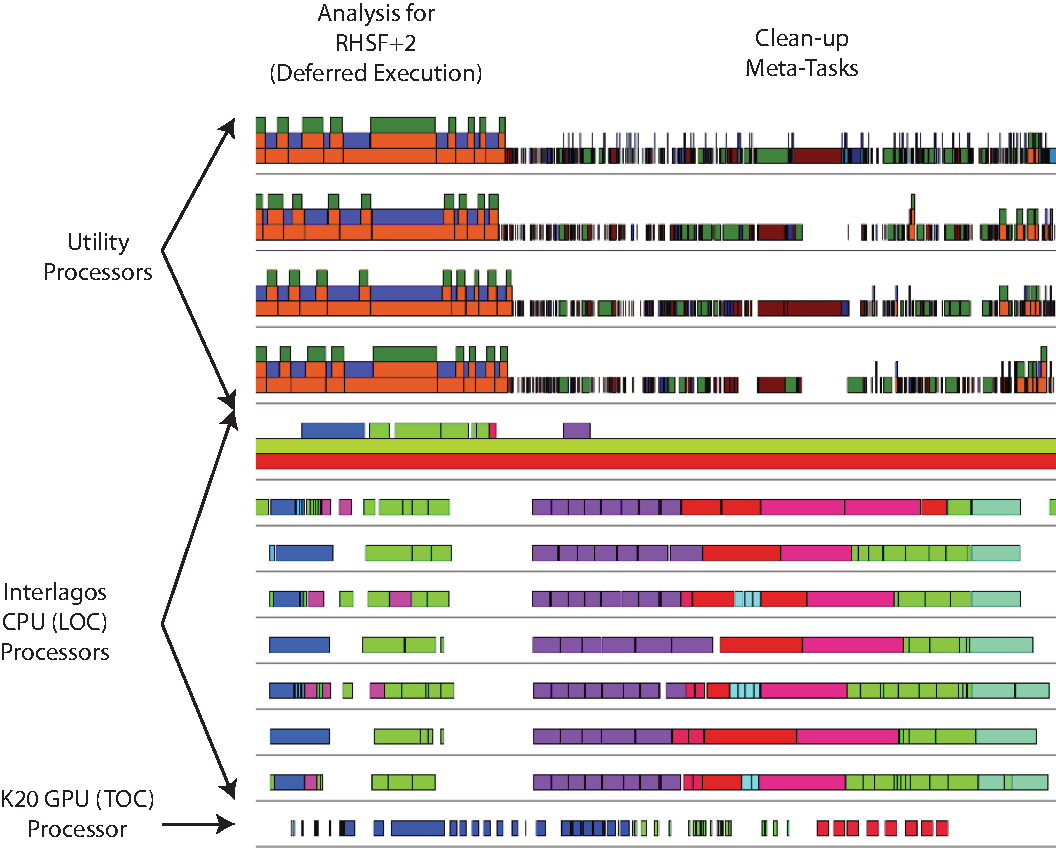
\includegraphics[scale=0.8]{figs/MixedMapping.pdf}
\caption{Example Mixed Mapping Strategy for S3D on a Titan Node\label{fig:mixedmap}}
\end{figure}

Ultimately, we referred to these two different
mapping approaches for S3D as {\em mixed} and
{\em all-GPU} mapping strategies. Figures~\ref{fig:mixedmap}
and \ref{fig:allgpumap} illustrate the differences
for the mixed and all-GPU mapping strategies
respectively. Each picture shows the performance of
the utility processors, CPUs, and GPUs on a single
Titan node for one RHSF invocation of the Heptane
mechanism\footnote{Interestingly, in the case of 
the utility processors, they are actually performing 
the dynamic analysis for the RHSF invocation that
occurs two steps later in the Runge-Kutta method.
This demonstrates the ability of Legion's deferred
execution model to permit the runtime to perform
analysis well in advance of where the actual
application is executing.}. In the mixed
strategy, the diffusive flux derivatives are computed
on the CPU-side of the PCI-E bus, leading to the
majority of the tasks that depend on those values
to also be mapped to CPU processors. Only the most
computationally expensive kernels (e.g. transport
and chemistry kernels) are mapped to the GPU. While
this leads to a relatively balanced workload between
CPUs and GPUs (depending on the relative performance
between the CPUs and GPUs), in general, the CPUs
are always busy while the GPUs are under-loaded.
The alternative approach is to map the diffusive
flux derivative computations onto GPU processors,
which generates the values in the framebuffer. This
then moves the majority of dependent tasks down 
to the GPU. Since both these tasks as well as the
computationally expensive tasks are all on the
GPU, the GPU processors are much more heavily
loaded, while the CPU processors have very few
tasks to perform (hence the all-GPU mapping name).

\begin{figure}
\centering
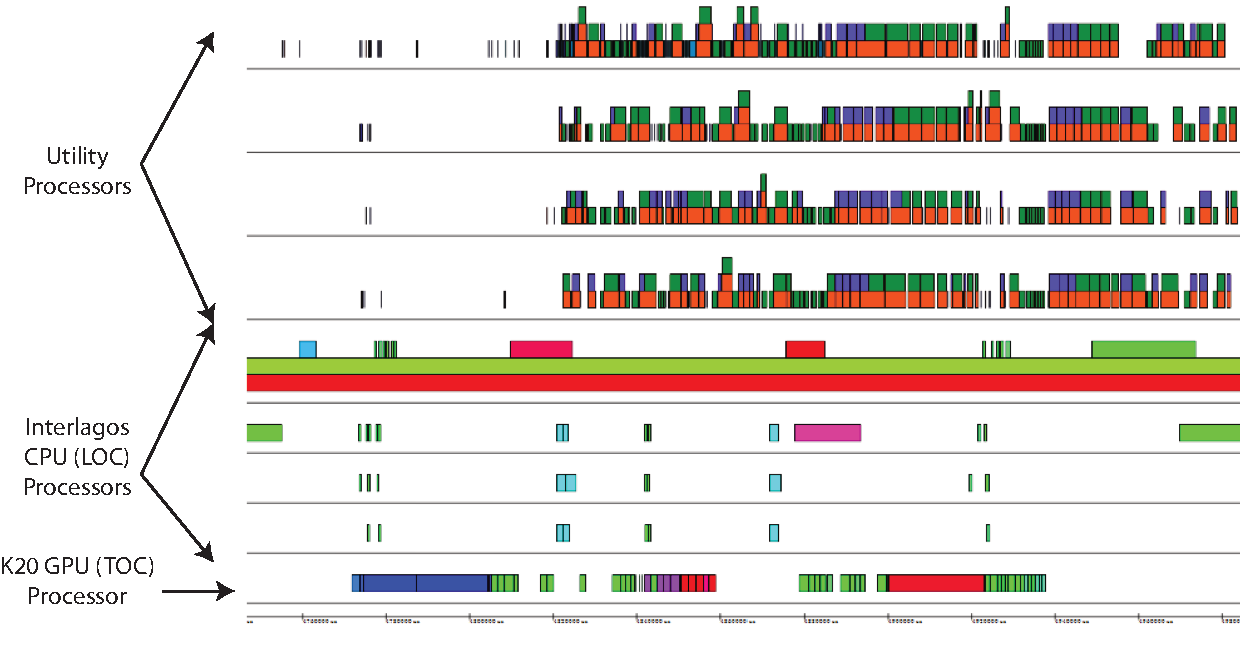
\includegraphics[scale=0.7]{figs/AllGPUMapping.pdf}
\caption{Example All-GPU Mapping Strategy for S3D on a Titan Node\label{fig:allgpumap}}
\end{figure}

Importantly, one commonly observed problem when
mapping code to accelerators also occurs in S3D.
In many cases, problem sizes are sometimes too
large to fit in the limited amount of framebuffer
memory for an accelerator\footnote{As of the writing
of this document, most accelerators have between
6 and 12 GB of either DRAM or GDDR5 memory.}. For
many codes, this will result in crashes due to 
out-of-memory errors. However, in the case of
Legion, it is easy to adjust to new larger
problem sizes with dynamic mapping strategies.
Figure~\ref{fig:largemap} shows an approach to 
mapping a $96^3$ cells per node Heptane problem onto
a Titan node. Only a limited number of tasks can
be mapped to the GPU as there is limited space in
the 6 GB framebuffer memory. Under this scenario,
the field-aware nature of Legion is crucial. Legion
understands precisely which fields are necessary for
executing the tasks mapped to the GPU, which means
only those fields are moved down to the GPU 
framebuffer. The mapper can therefore dynamically 
manage the working set of the GPU and ensure that
the code can run unlike the case today where 
significant refactoring would be required.

\begin{figure}
\centering
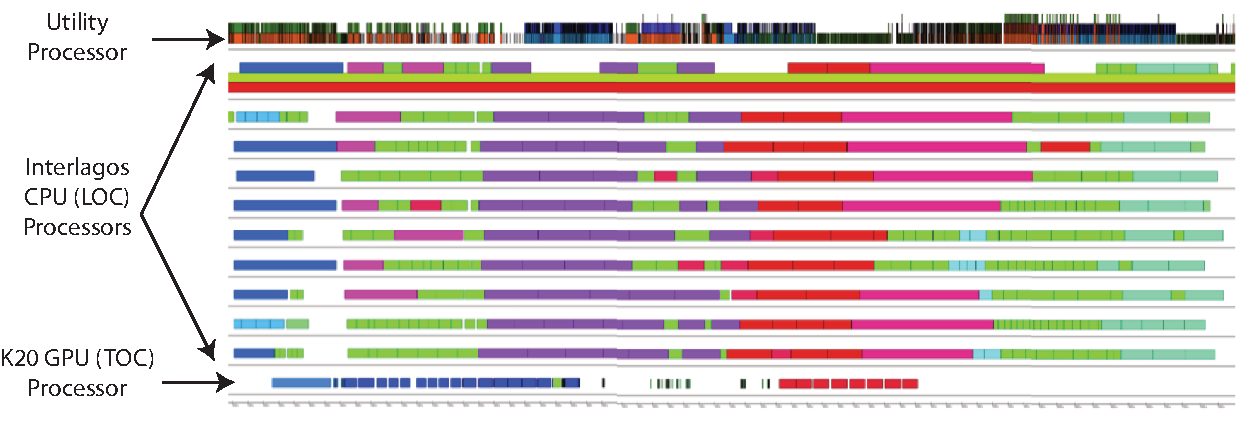
\includegraphics[scale=0.7]{figs/LargeMapping.pdf}
\caption{Mapping Strategy for a Large S3D Problem Size\label{fig:largemap}}
\end{figure}

The crucial insight provided by our experience 
mapping S3D is that we would never have discovered
either of these mapping strategies without the
decoupled nature of the Legion mapping interface.
We tried more than a hundred different mapping 
implementations before settling on the two primary 
approaches described above. The Legion mapping 
interface provided the flexibility to try many
different mapping strategies without having to be 
concerned with correctness. Furthermore, as we will
show in Section~\ref{sec:s3dperf}, the determination
of which mapping strategy performs better is 
architecture dependent.

\section{Performance Results}
\label{sec:s3dperf}
In order to evaluate our implementation of S3D in
Legion, we ran experiments on two different
supercomputers: Keeneland \cite{Keeneland} and 
Titan \cite{Top500}. Keeneland is a 250 node cluster
with an Infiniband interconnect. Each Keeneland
node contains 2 CPU sockets with an 8-core Intel
Sandybridge chip in each socket, 3 NVIDIA Fermi
M2090 GPUs, and 32 GB of DRAM partitioned between
the two sockets. Titan is the number two supercomputer
in the world (as of the writing of this document)
consisting of more than 18000 nodes with a Cray
Gemini Interconnect. Each Titan node has one CPU
socket with a 16-core AMD Interlagos chip, one
NVIDIA Kepler K20 GPU, and 32 GB of DRAM partitioned
across four primary Interlagos NUMA domains.
There is an interesting mismatch between CPU and
GPU pairings as we will see. The CPUs and GPUs
on Keeneland are relatively evenly matched, while
on Titan there is a difference of several generations
between the CPU cores and GPU cores. These differences
will show different performance under different
mapping strategies as we will observe.

For both or our target machines, we experimented 
with three different chemical mechanisms (DME, Heptane,
and PRF) for three different problem sizes. The numerical
formulation of the S3D simulation is designed for 
weak-scaling (keeping a fixed problem size per node 
and trying to maintain uniform throughput per node). 
For the DME and Heptane mechanisms, we experimented
with problem sizes of $48^3$, $64^3$, and $96^3$ cells
per node.  For the larger PRF mechanism we used smaller
problem sizes of $32^3$, $48^3$, and $64^3$ cells per
node. For different problem sizes, we also experimented
with each of our two mapping strategies.

% Re-ranking
To test for weak scaling we ran experiments starting 
with one node and scaling up by powers of two. (Our
implementation of Legion S3D performs equally well 
for node counts that are not powers of two.) For
Keeneland, we show scaling through 128 nodes, while
for Titan we show scaling through 8192 nodes. As a
baseline version, we use the combination OpenACC
and MPI version of S3D that was independently 
hand optimized by engineers from NVIDIA and Cray
over the course of a year. 

For all experiments run on 1024 nodes or more, we 
found that a node re-ranking script was necessary 
for taking into account network topology performance 
effects. We use the genetic algorithm re-ranking script 
described in \cite{GAMPI} to perform the re-ranking.
The script uses a genetic algorithm to discover 
better assignments of ranks to nodes to minimize
latency for S3D (and applications with a nearest 
neighbors communication pattern). While we could
have computed a topologically aware re-ranking in our
custom S3D Legion mappers, we use the same re-ranking script
for both MPI/OpenACC and Legion versions of S3D so
we can compare the latency hiding abilities of
both versions directly.

\begin{figure}
\centering
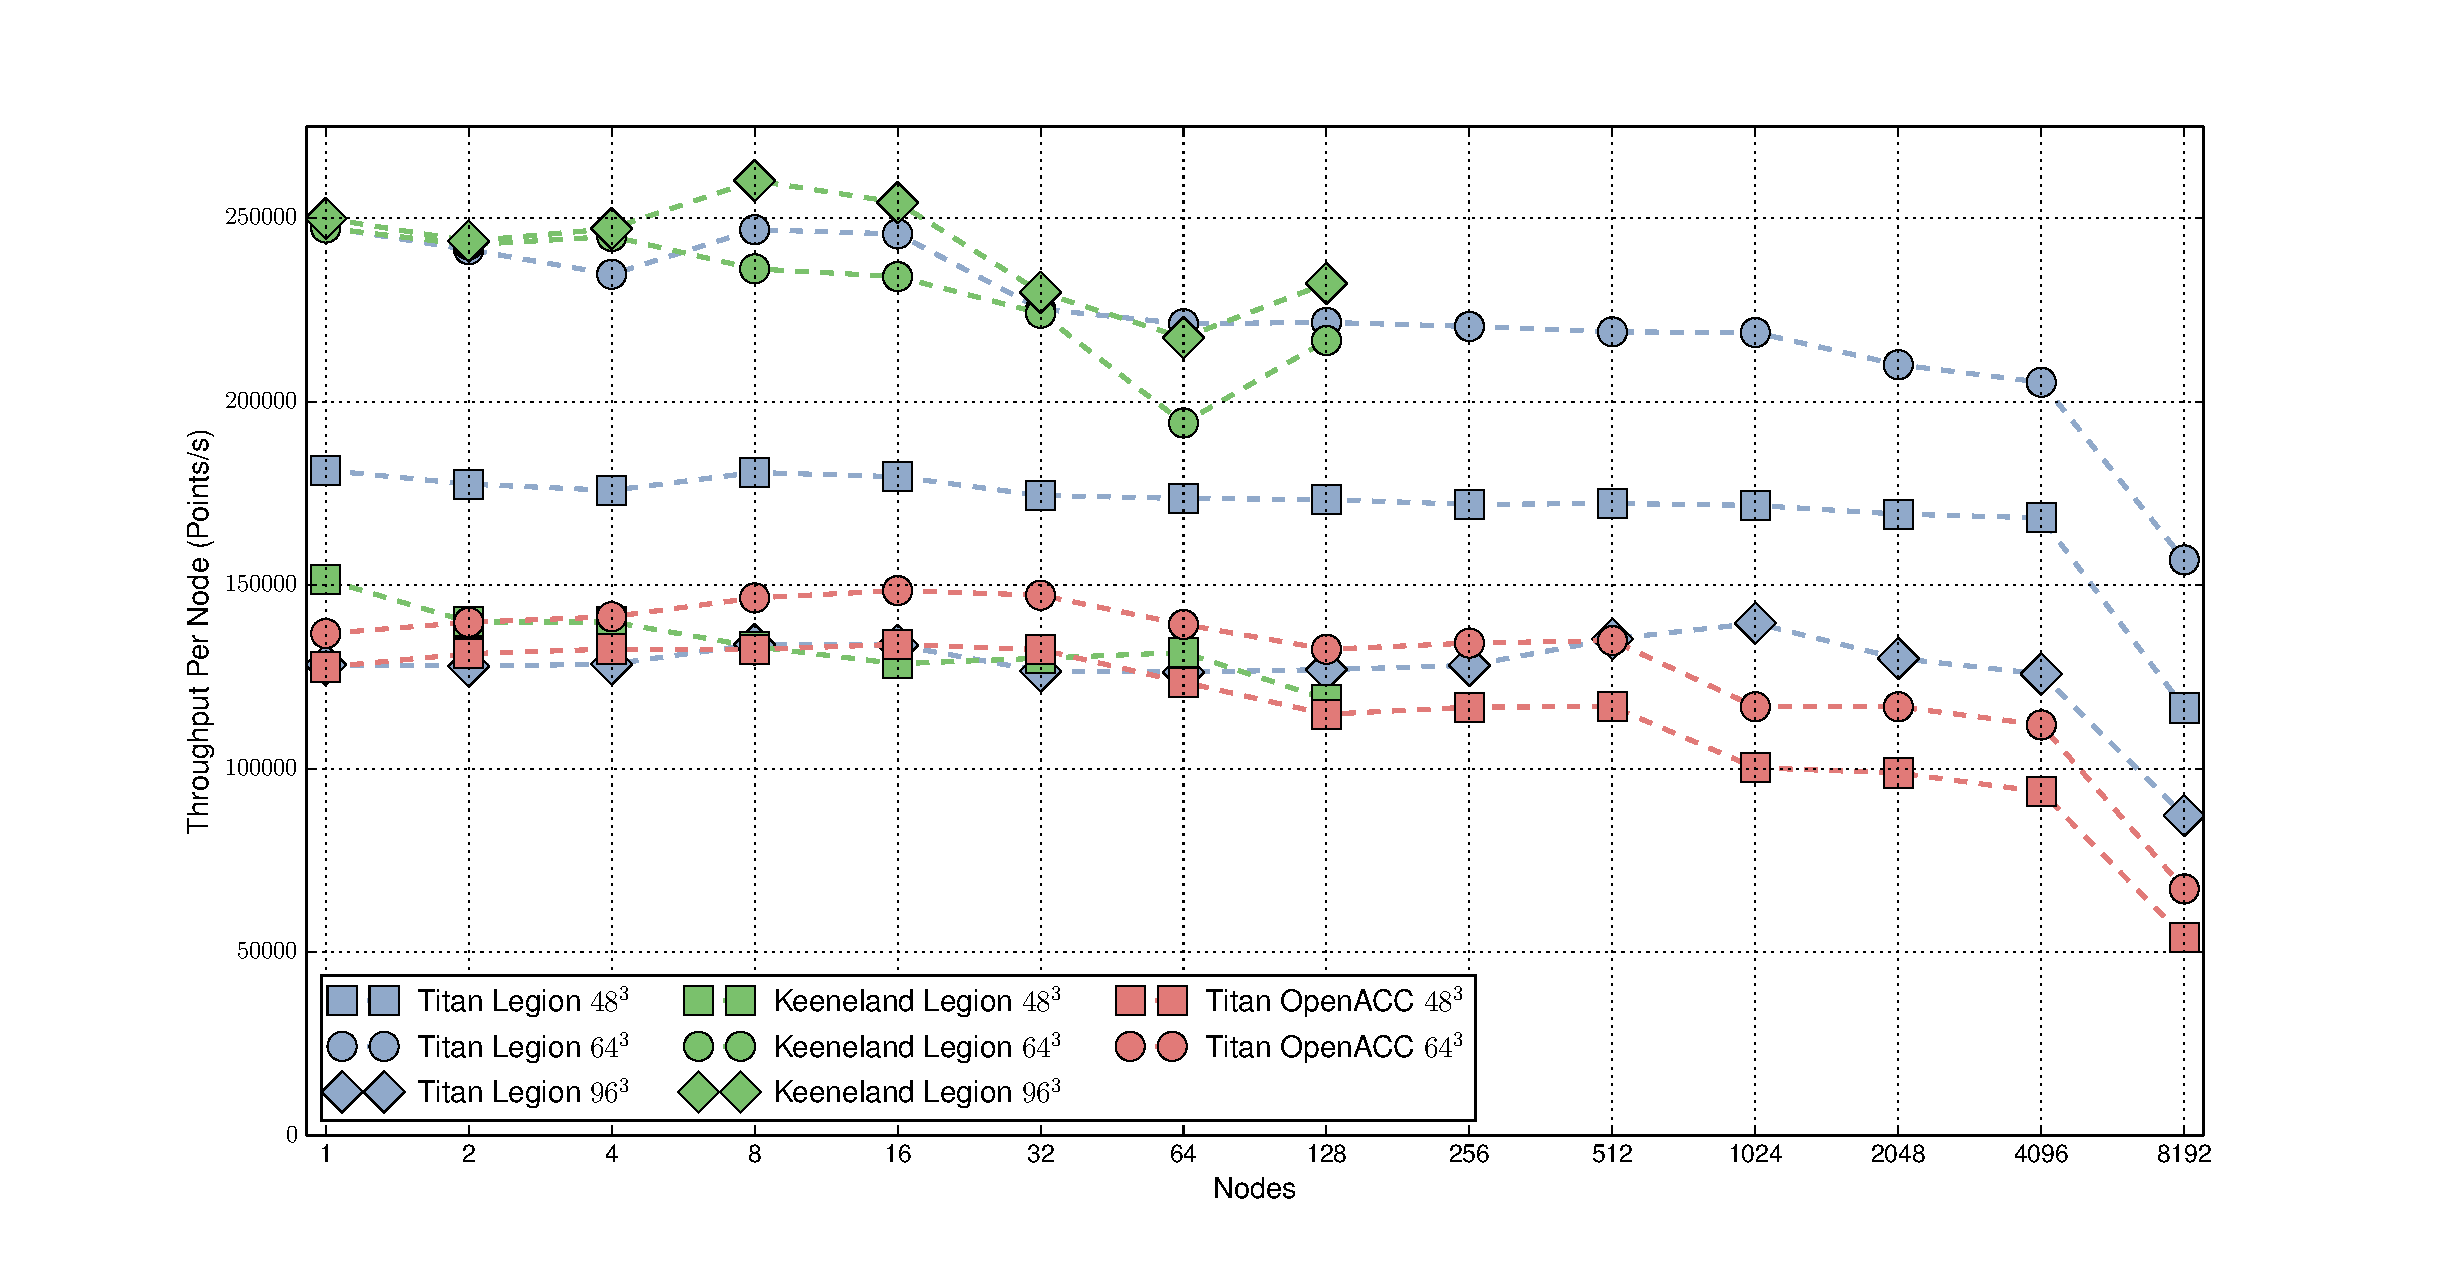
\includegraphics[scale=0.4]{figs/dme_scaling.pdf}
\caption{S3D Weak Scaling Performance for DME Mechanism\label{fig:dmescale}} 
\end{figure}

Figures~\ref{fig:dmescale} and \ref{fig:heptscale} 
plot the per-node throughput of the 
DME and Heptane mechanisms respectively for several 
different problem sizes on both the Titan and Keeneland 
supercomputers. Higher lines show better performance 
and flat lines are indicative of good weak scaling (tail-offs 
are inefficiencies). For the Legion runs, performance at a 
given problem size is shown for the best performing 
mapping strategy. On Keeneland, the best mapping strategy
is to use the mixed CPU-GPU approach to leverage the 
relatively balanced computational capabilities of the 
CPUs and GPUs. On Titan, the best mapping strategy is 
to use the all-GPU approach due to the extreme imbalance 
between the CPUs and the GPUs: the Kepler K20 GPU is many
times more powerful than all the Bulldozer CPU cores combined.
One important detail is that because the MPI-OpenACC
version of the code effectively has its mapping hard-coded
to place the majority of work on the GPU, it is unable
to run a $96^3$ problem size without exhausting the
available memory in the GPU framebuffer.

\begin{figure}
\centering
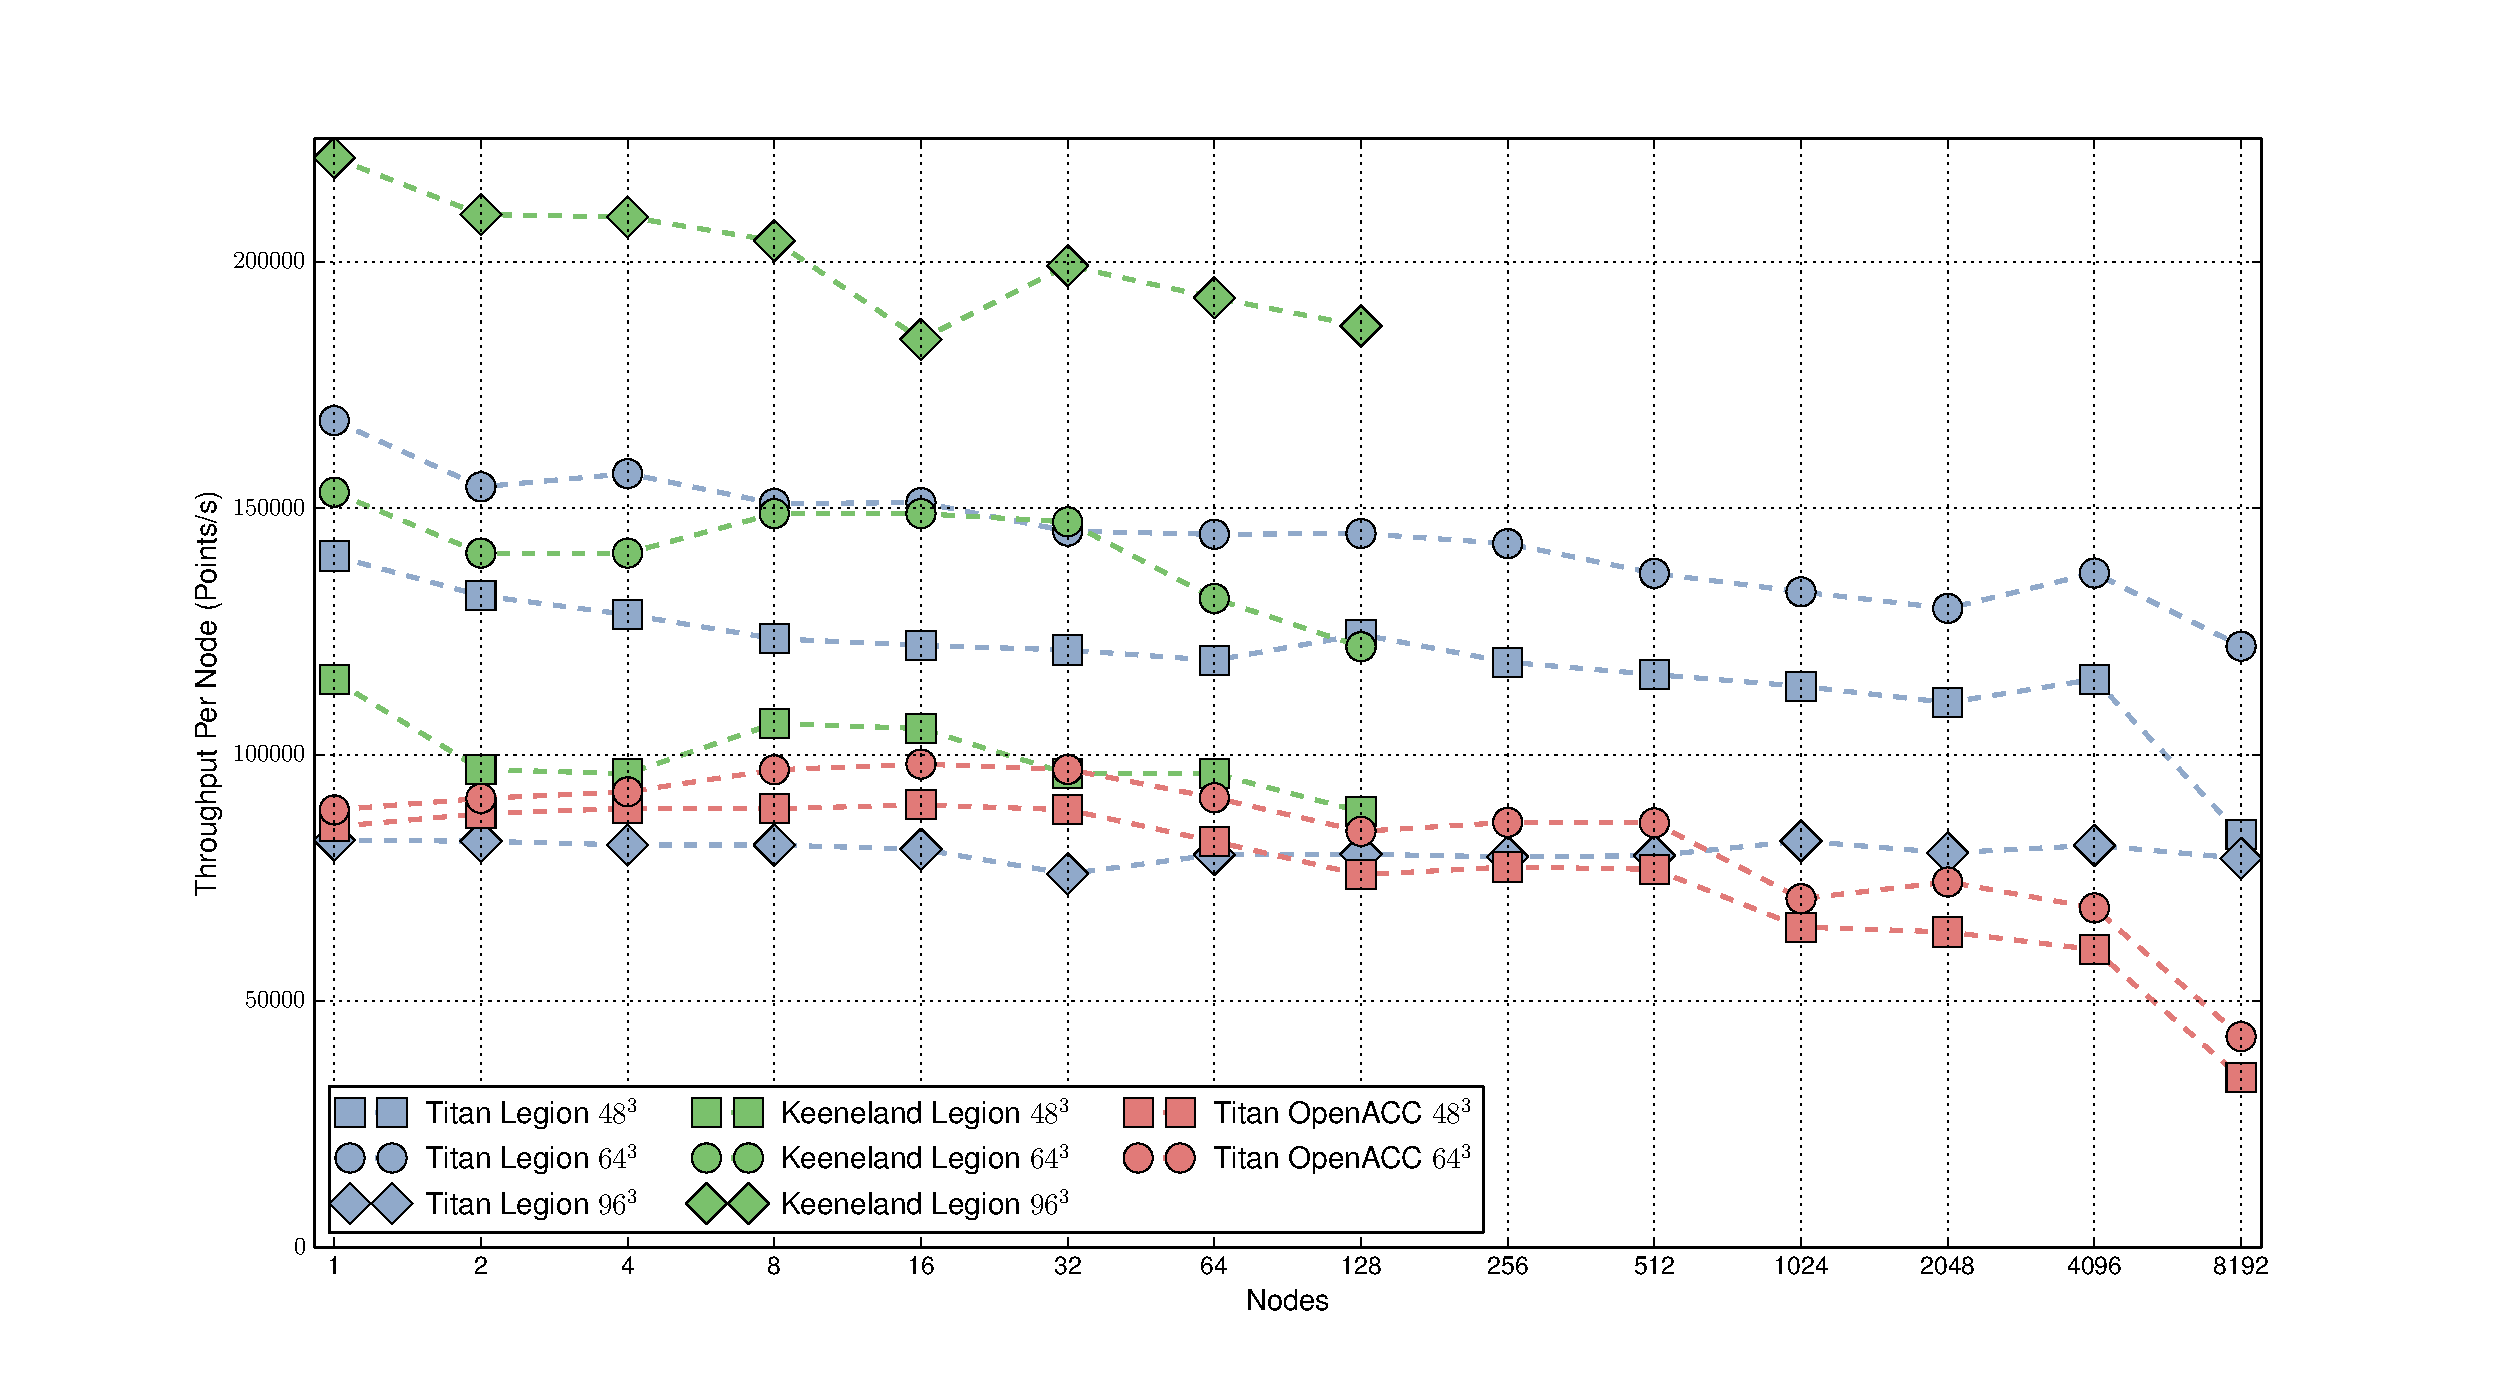
\includegraphics[scale=0.4]{figs/hept_scaling.pdf}
\caption{S3D Weak Scaling Performance for Heptane Mechanism\label{fig:heptscale}}
\end{figure}

As we can see in Figures~\ref{fig:dmescale} and 
\ref{fig:heptscale}, in general larger 
problem sizes achieve higher throughput as both the MPI-OpenACC
and Legion versions of S3D can use the additional work to
better overlap computation and communication. The one 
exception to this trend is with the $96^3$ problem size
for Legion on Titan. In this case, in order to fit the 
problem size within a Titan node, we had to use the
mixed CPU-GPU mapping, which is not as efficient due to
the slow Bulldozer CPU cores. We therefore notice a fall
off in performance compared to the $64^3$ problem size.

Overall, Legion significantly outperforms the MPI-OpenACC
code. Between 1024 and 8192 nodes, when compared to the
MPI-OpenACC code, the Legion version of S3D is 1.71-2.33X 
faster for the DME mechanism and 1.75-2.85X faster for
the Heptane mechanism. On the Heptane mechanism, Legion
does particularly well at discovering additional parallel
work and using it to better overlap computation and
communication (both inter-node as well as intra-node over 
the PCI-E bus). Both the Legion and MPI-OpenACC versions
experience a falloff in performance at 8192 nodes. This
is due to the failure of the genetic algorithm re-ranking
script to fully explore the space of possible re-rankings
given a fifteen minute time limit. Interestingly, for the
Heptane mechanism, Legion is able to mitigate this effect
by discovering further work to hide the additional latency.
Note that this effect is even more pronounced for larger
problem sizes.

\begin{figure}
\centering
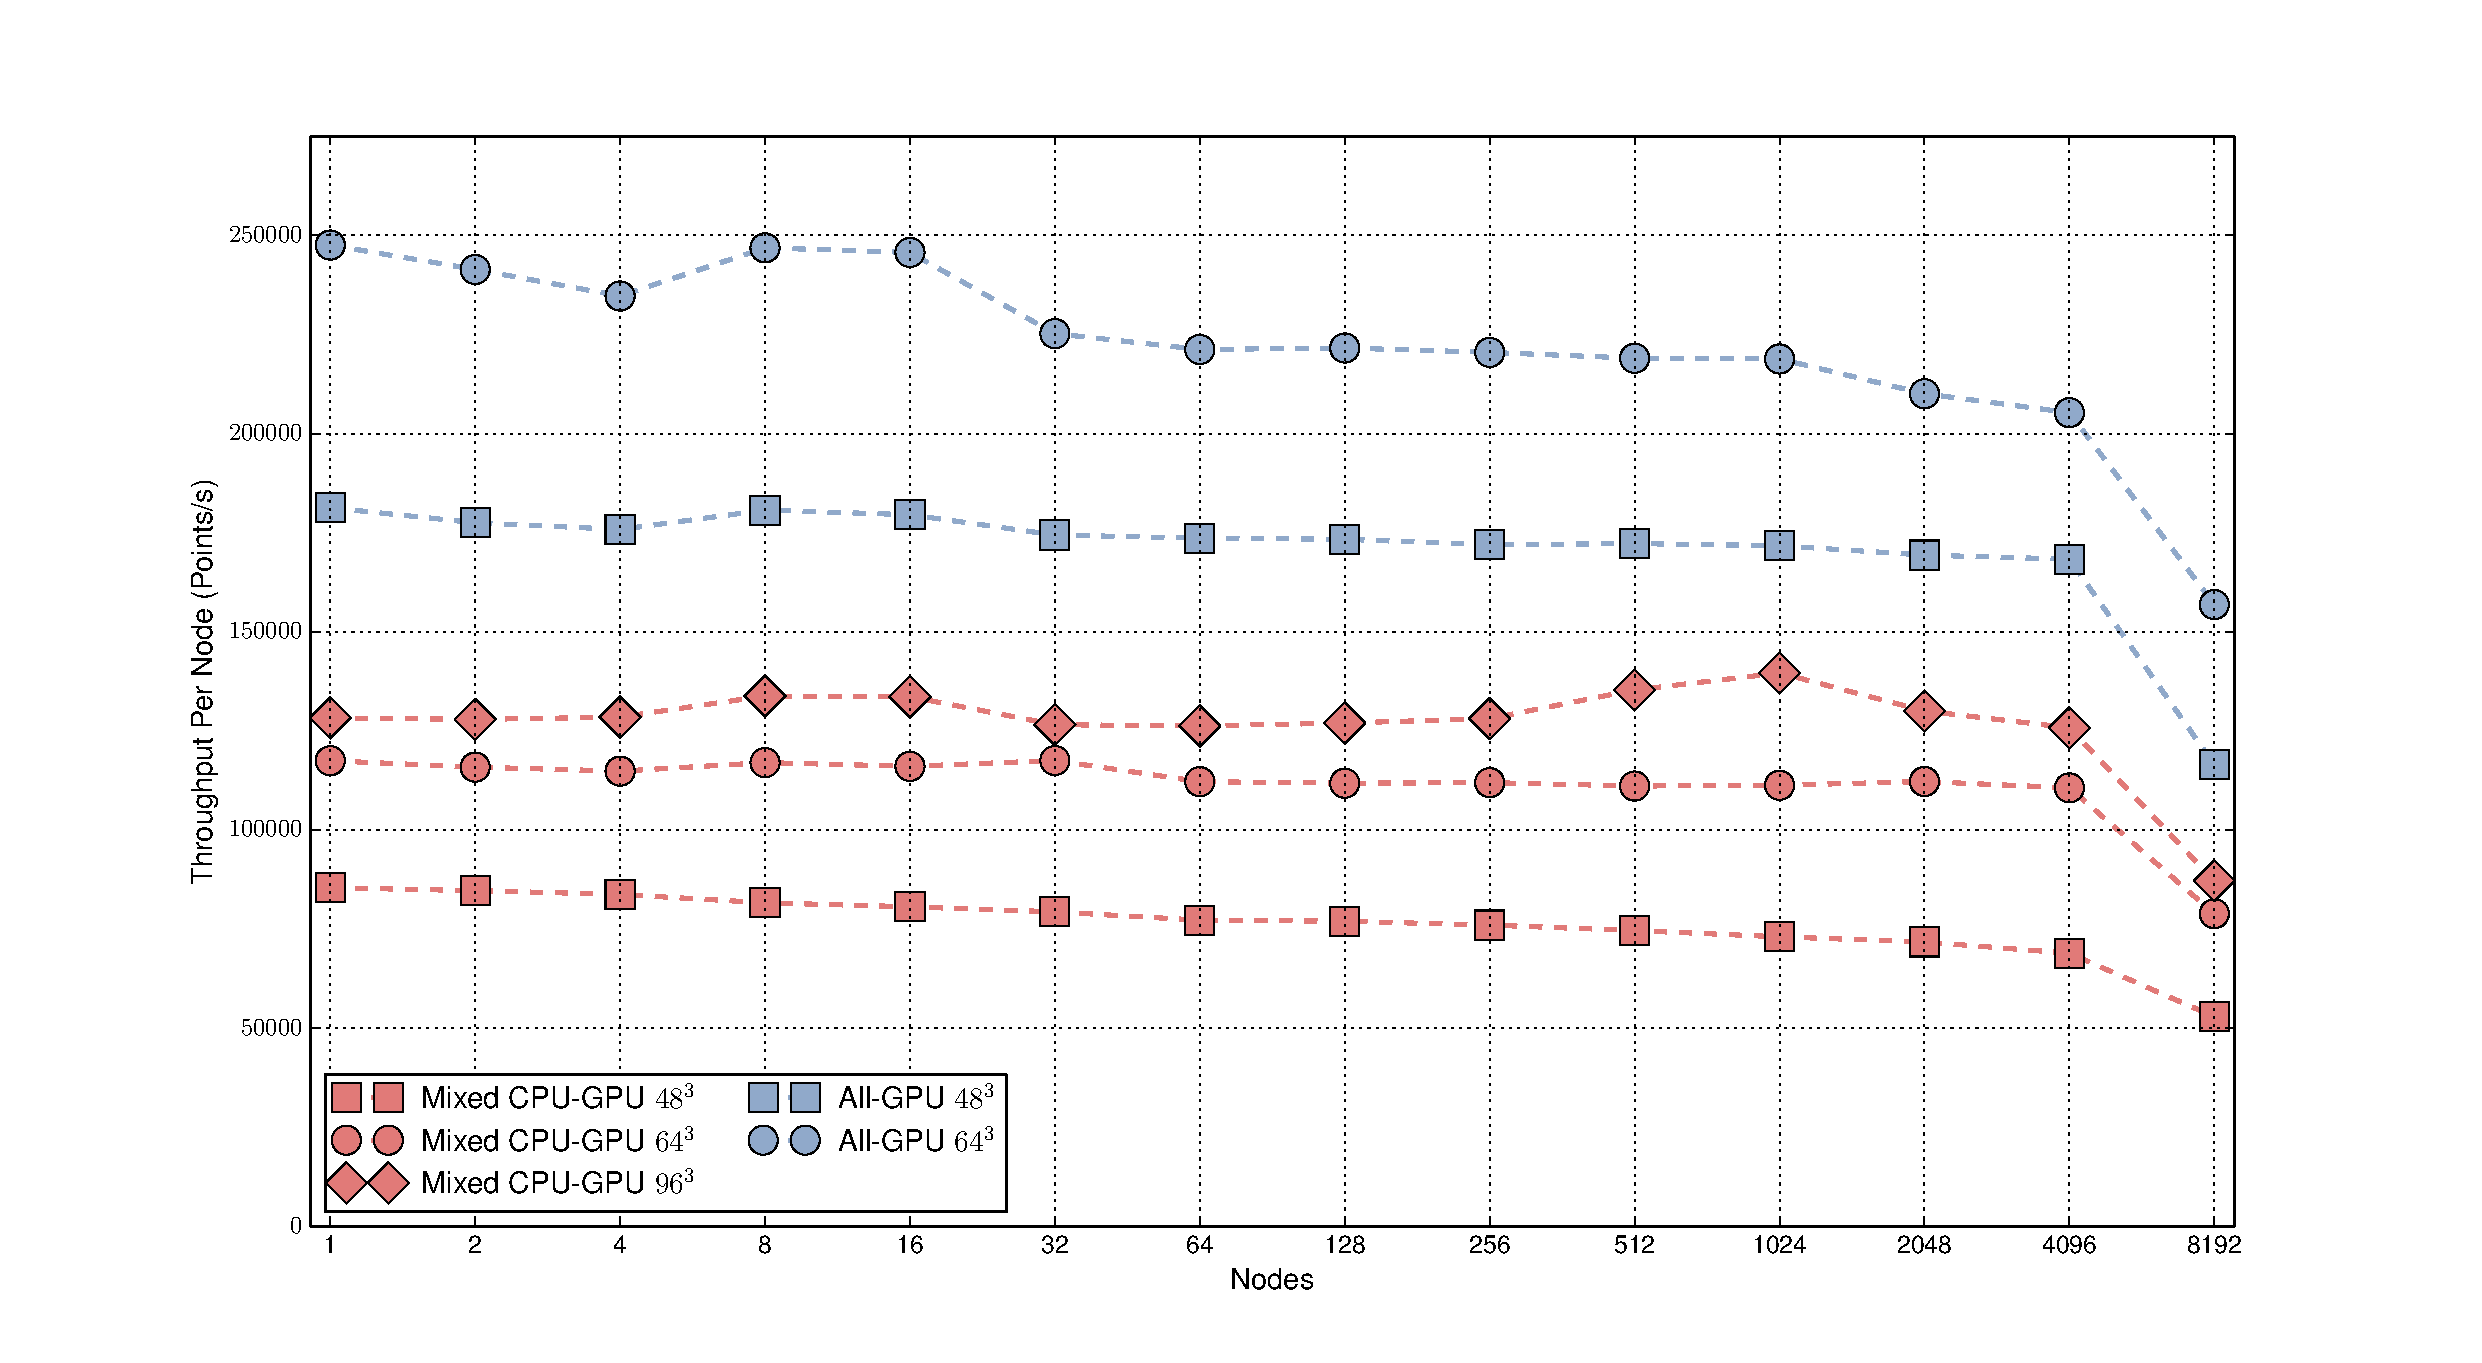
\includegraphics[scale=0.4]{figs/legion_dme_titan.pdf}
\caption{Mapping Strategies for the S3D DME Mechanism\label{fig:dmemap}}
\end{figure}

Figures~\ref{fig:dmemap} and \ref{fig:heptmap} 
illustrate the performance of different 
Legion mapping strategies for all problem sizes on Titan.
On Titan, the severe performance mismatch between the CPUs 
and the GPUs results in the best mapping being to place as
much work as possible on the GPUs. In contrast, on Keeneland,
the best mapping strategy is always to evenly distribute work
between CPUs and GPUs to ensure that all processing elements
are fully utilized. Mismatches in processor capabilities are
just another form of heterogeneity that programmers need to
contend with as part of writing code for current and future
architectures. By leveraging the Legion mapping interface
we were easily able to deal with this form of heterogeneity
without needing to make any code changes to the machine
independent Legion code; we simply wrote different 
mappers for Titan and Keeneland.

\begin{figure}
\centering
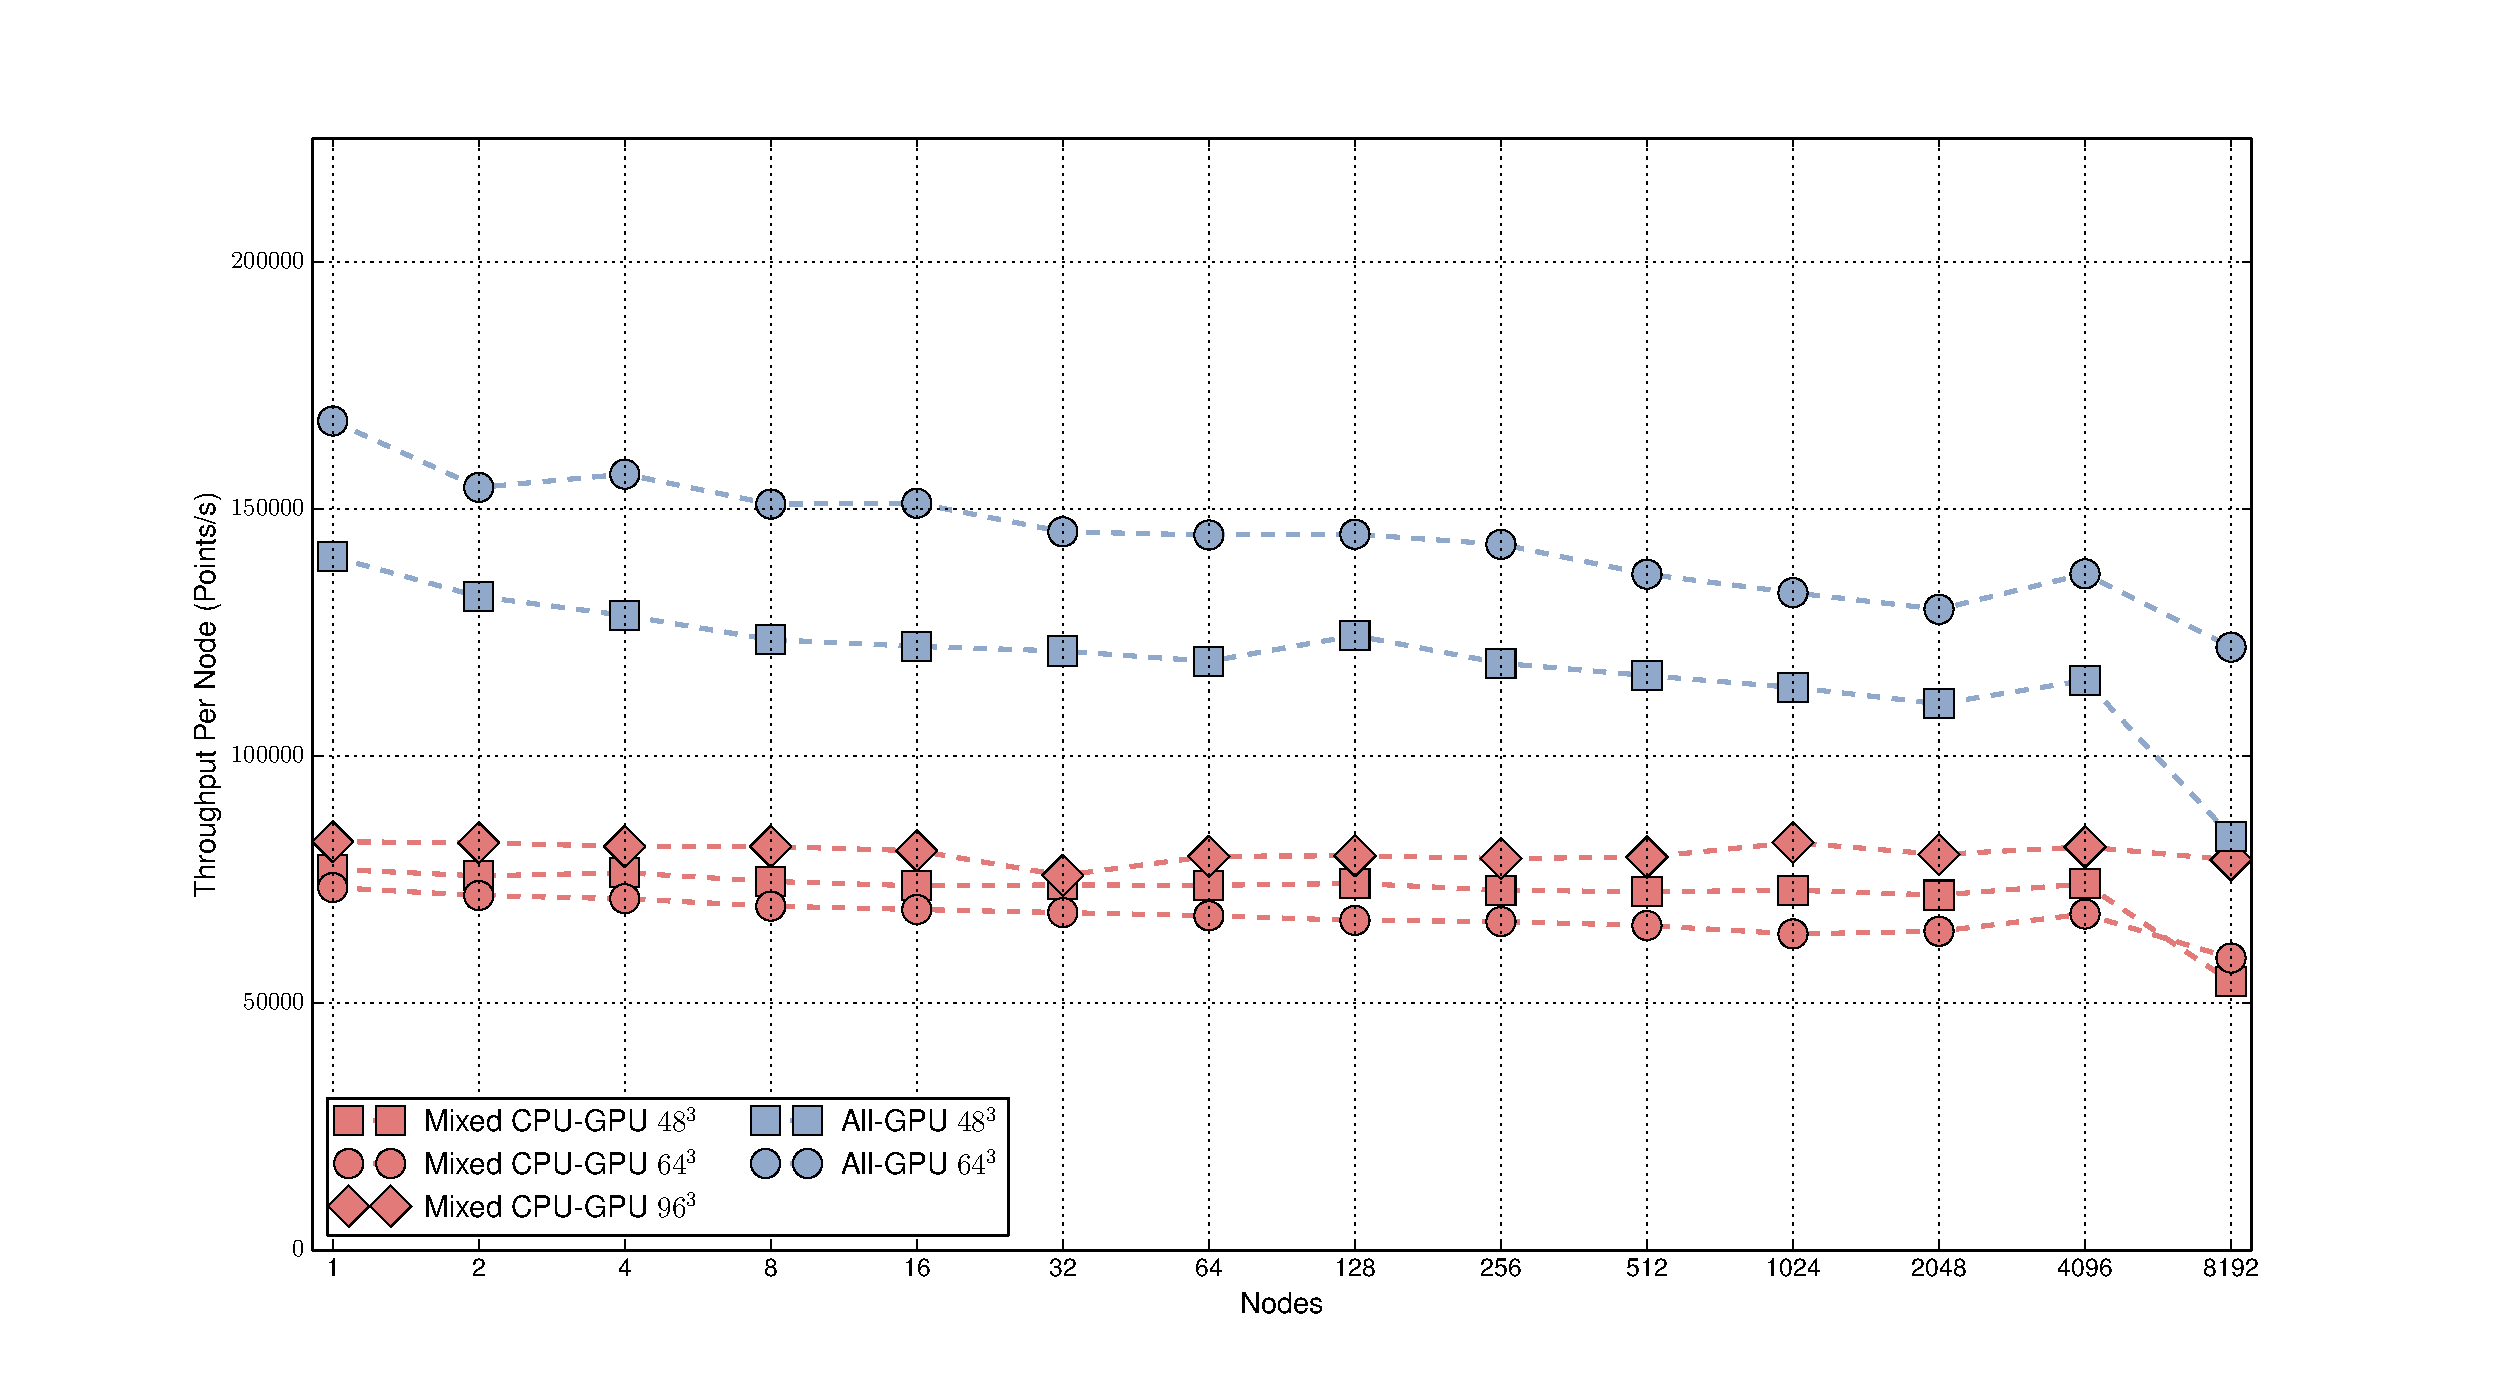
\includegraphics[scale=0.4]{figs/legion_hept_titan.pdf}
\caption{Mapping Strategies for the S3D Heptane Mechanism\label{fig:heptmap}}
\end{figure}

In addition to the performance gains on existing mechanisms,
Legion is also able to support the PRF mechanism that is much 
larger than the DME and Heptane mechanisms currently supported 
by the MPI-OpenACC code. Each new mechanism that is significantly 
different in size or computational intensity requires the 
MPI-OpenACC code to be refactored in order to tune for performance, 
often necessitating many man hours of work. Our Legion version of
S3D requires no refactoring and only slight modifications
to the customized mapper (no more than 10 lines of code). (We
do use the Singe DSL compiler to generate new leaf task kernel 
implementations for the additional chemistry, but the base 
S3D code is unmodified.) Figure~\ref{fig:prfperf} shows performance results
for the PRF mechanism running on Titan for three different
problem sizes with different mapping options. Note that, unlike
smaller mechanisms, there is no performance cliff at 8192 nodes
for the PRF mechanism, as Legion is able to discover sufficient 
work in the PRF mechanism to automatically hide all of the 
communication latency. Being able to adapt to new mechanisms and 
automatically scale with just a few changes to a custom mapper 
truly illustrates the power of the Legion programming model.

\begin{figure}
\centering
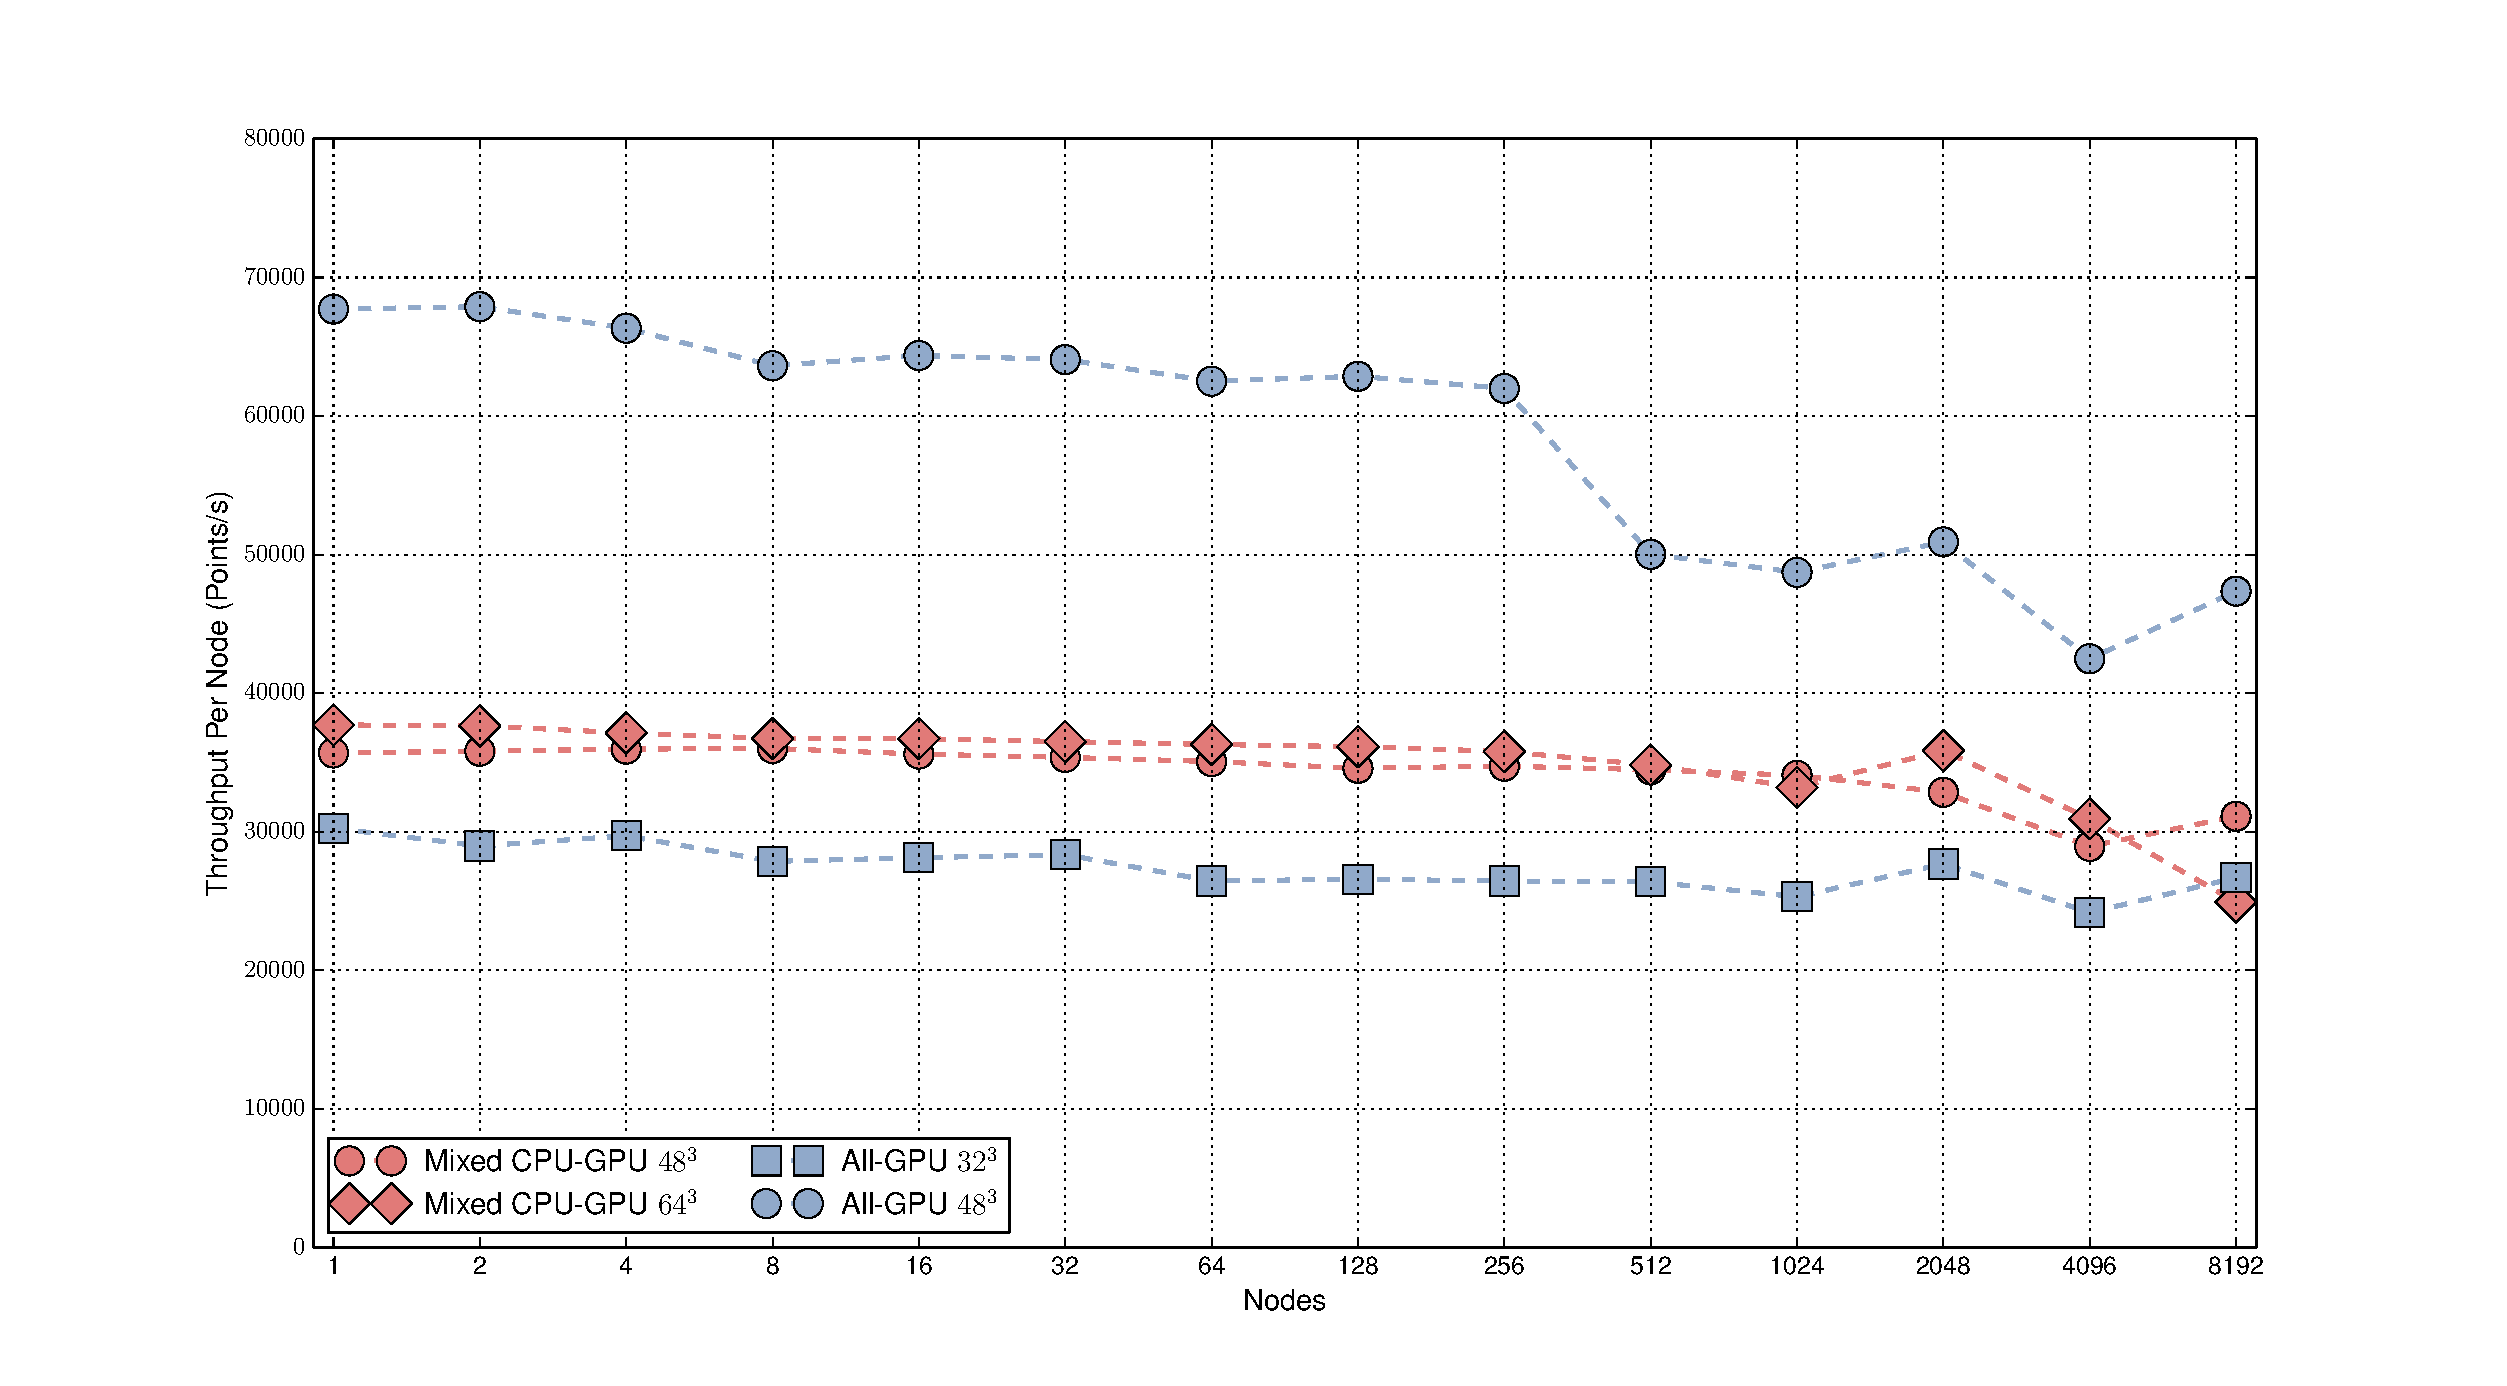
\includegraphics[scale=0.4]{figs/legion_prf_titan.pdf}
\caption{Performance of Legion S3D for PRF Mechanism\label{fig:prfperf}}
\end{figure}

\section{Programmability}
\label{sec:s3dprogram}

The final criteria on which we evaluate our Legion implementation
of S3D is programmability. While this is qualitative metric, it 
is an important one, as the cost of programmer productivity and
software maintenance can often exceed the cost of doing production
runs. In the process of tuning our Legion version of S3D for both
the Titan and Keeneland machines, we were able to try hundreds of
different mapping strategies all without needing to modify the 
machine-independent specification of S3D. This demonstrates the
power of our core Legion design goal to decouple an application 
specification from its mapping. In the future, we anticipate this
property will allow us to easily port S3D to new architectures
simply by developing new mapping strategies.

